\documentclass[a4paper,10pt]{article}

% ---------- Encodage et langue
\usepackage[utf8]{inputenc}
\usepackage[T1]{fontenc}
\usepackage[french]{babel}

% ---------- Police : Palatino + math assorti (académique, lisible)
\usepackage{mathpazo}
\linespread{1.05}

% ---------- Mise en page
\usepackage[margin=2cm,top=1.8cm,bottom=2cm]{geometry}
\usepackage{microtype}
\usepackage{parskip}
\setlength{\parskip}{4pt}

% ---------- Math, figures, tableaux
\usepackage{amsmath,amssymb}
\usepackage{graphicx}
\usepackage{booktabs}
\usepackage{caption}
\usepackage{subcaption}
\usepackage{array}
\usepackage{xcolor}
\definecolor{accent}{HTML}{C8102E}        % rouge EPFL
\definecolor{ink}{HTML}{1D3557}           % bleu marine
\definecolor{soft}{HTML}{6C7A89}          % gris

\captionsetup{font=small,labelfont={bf,color=accent},
              labelsep=period,skip=4pt}

% ---------- Code
\usepackage{minted}
\setminted{
  fontsize=\footnotesize,
  frame=single,
  framesep=4pt,
  rulecolor=\color{soft!40},
  bgcolor=gray!4,
  linenos=false,
  breaklines=true,
  style=friendly,
}

% ---------- Liens
\usepackage[colorlinks=true,
            urlcolor=ink,
            linkcolor=ink,
            citecolor=ink]{hyperref}

% ---------- Hiérarchie titres
\usepackage{titlesec}
\titleformat{\section}
  {\Large\bfseries\color{accent}}
  {\thesection.}{0.6em}{}
\titleformat{\subsection}
  {\normalsize\bfseries\color{ink}}
  {\thesubsection.}{0.4em}{}
\titlespacing*{\section}{0pt}{12pt}{4pt}
\titlespacing*{\subsection}{0pt}{8pt}{2pt}

% ---------- En-tête / pied de page
\usepackage{fancyhdr}
\pagestyle{fancy}
\fancyhf{}
\fancyhead[L]{\small\color{soft}Projet 5, Flexion d'une poutre 2D}
\fancyhead[R]{\small\color{soft}CIVIL-321}
\fancyfoot[C]{\small\color{soft}\thepage}
\renewcommand{\headrulewidth}{0pt}

\title{\vspace{-2em}%
  {\LARGE\bfseries\color{ink} Projet 5\,: flexion d'une poutre 2D}\\[3pt]
  {\large T3, T6 iso-paramétriques et comparaison à Euler-Bernoulli}}
\author{\normalsize Hugo Gebel\\[1pt]
        \small\color{soft} CIVIL-321, Modélisation Numérique des Solides et Structures}
\date{\small\color{soft}\today}

\begin{document}
\maketitle
\thispagestyle{fancy}

\noindent\colorbox{ink!5}{%
\begin{minipage}{\dimexpr\linewidth-2\fboxsep}\small
\textbf{Résumé.} On étend un code éléments finis 2D linéaire (T3) à
l'élément T6 quadratique iso-paramétrique. L'implémentation passe le
patch test à $\sim 10^{-19}$ sur géométrie distordue. Une poutre
encastrée-appuyée sous charge répartie est ensuite résolue avec T3 et
T6, puis confrontée à la théorie d'Euler-Bernoulli sur la flèche, la
contrainte de flexion, la convergence en $h$ et les fréquences propres.
Le shear locking observé sur T3 est diagnostiqué et la résolution par
T6 est démontrée numériquement.\\[2pt]
\textit{Code et notebook reproductibles\,:}
\href{https://github.com/hugogebel-boop/mnss-projet-flexion}{\texttt{github.com/hugogebel-boop/mnss-projet-flexion}}
\end{minipage}}

% =========================================================================
\section{Implémentation T6}

\subsection{Fonctions de forme et dérivées}
L'élément T6 est un triangle quadratique à 6 nœuds, 3 sommets et 3 nœuds
médians sur arêtes (convention gmsh). Avec les coordonnées d'aire
$L_1 = 1{-}s{-}t$, $L_2 = s$, $L_3 = t$\,:
\[
\begin{array}{ll}
N_1 = L_1(2L_1{-}1) & N_4 = 4 L_1 L_2\\[1pt]
N_2 = L_2(2L_2{-}1) & N_5 = 4 L_2 L_3\\[1pt]
N_3 = L_3(2L_3{-}1) & N_6 = 4 L_3 L_1
\end{array}
\]
La matrice de gradients naturels $C(s,t)\in\mathbb{R}^{4\times 12}$
regroupe les dérivées $\partial N_i/\partial s$ et $\partial N_i/\partial t$.

\subsection{Matrice $B$ et Jacobienne}
Le pattern iso-paramétrique reste celui du T3, seules les tailles
changent ($B\in\mathbb{R}^{3\times 12}$)\,:
\begin{equation}
B(s,t) \;=\; A\;J_\text{block}^{-1}(s,t)\;C(s,t),
\quad
A = \begin{pmatrix} 1&0&0&0\\0&0&0&1\\0&1&1&0\end{pmatrix},
\quad
J_\text{block} = \begin{pmatrix} J&0\\0&J\end{pmatrix}.
\end{equation}
La Jacobienne $J=[\partial(x,y)/\partial(s,t)]$ se calcule par le
principe iso-paramétrique $\tilde\nabla(x,y) = C\cdot\{x_i,y_i\}$.

\subsection{Quadrature de Gauss}
Trois règles sont implémentées (somme des poids $= \tfrac12$,
l'aire du triangle de référence). Un point pour T3 (degré 1 exact),
trois points pour $K^\text{T6}$ avec $B$ linéaire (degré 2 exact),
sept points pour la masse T6 (degré 5, $N^TN$ étant de degré 4).

\begin{minted}{python}
def gauss_triangle(npts):
    if npts == 1:                       # T3, K (B et J constants)
        return [(1/3, 1/3)], [1/2]
    if npts == 3:                       # T6, K (B linéaire)
        return [(1/6, 1/6), (2/3, 1/6), (1/6, 2/3)], [1/6]*3
    if npts == 7:                       # T6, M (N quadratique)
        a1, a2 = 0.0597158717, 0.4701420641
        w0, w1, w2 = 0.225/2, 0.1323941527/2, 0.1259391805/2
        quads = [(1/3, 1/3),
                 (a1, a1), (1-2*a1, a1), (a1, 1-2*a1),
                 (a2, a2), (1-2*a2, a2), (a2, 1-2*a2)]
        return quads, [w0, w1, w1, w1, w2, w2, w2]
\end{minted}

\subsection{Assemblage}
Le code dispatche sur \texttt{connectivite.shape[1]} (3 ou 6) pour
choisir le bon couple (\texttt{calculerBetJ}, $n_\text{dof}$).
L'assemblage utilise \texttt{scipy.sparse} (COO\,$\to$\,CSR), ce qui
évite la saturation mémoire jusqu'à $\sim\!10^5$~DDL.

% =========================================================================
\section{Validation\,: patch test}

On teste les deux éléments sur la géométrie de la fig.~10 du sujet
(carré $[0,L]\times[0,h]$ découpé en 4 triangles autour d'un nœud
central excentré en $(0.6L,\,0.55h)$). Les nœuds médians T6, placés au
milieu géométrique des arêtes, héritent du décalage. La transformation
iso-paramétrique n'est donc pas affine, ce qui rend le test
discriminant.

On impose le champ de déplacement linéaire correspondant à un état
$(\varepsilon,\sigma)$ uniforme sur les nœuds frontières (Dirichlet
inhomogène) et on résout $K_{ii}\,u_i = -K_{ib}\,u_b$ pour les nœuds
intérieurs. L'erreur sur les déplacements et sur la déformation aux
points de Gauss doit alors tendre vers la précision machine.

\begin{figure}[!ht]
\centering
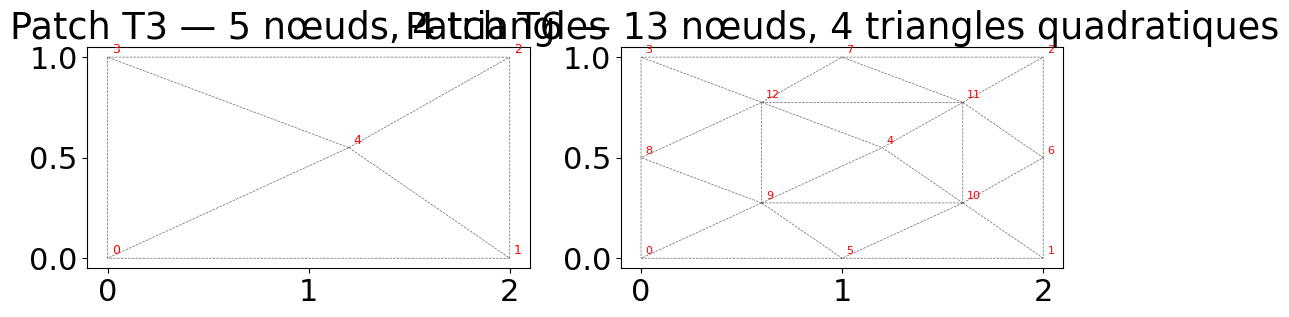
\includegraphics[width=0.78\linewidth]{figures/patch_meshes.png}
\caption{Maillages de la fig.~10. T3 (5 nœuds) à gauche, T6 (13 nœuds)
à droite. Le décalage du nœud central rend la transformation
iso-paramétrique non affine.}
\label{fig:patch}
\end{figure}

\begin{table}[!ht]
\centering\small
\renewcommand{\arraystretch}{1.15}
\begin{tabular}{lcccc}
\toprule
                  & T3 traction & T3 cisaillement & T6 traction & T6 cisaillement\\
\midrule
err.\ déplacement & $1.4\!\times\!10^{-20}$ & $5.4\!\times\!10^{-20}$
                  & $2.2\!\times\!10^{-19}$ & $1.1\!\times\!10^{-19}$\\
err.\ déformation & $2.2\!\times\!10^{-19}$ & $2.2\!\times\!10^{-19}$
                  & $8.7\!\times\!10^{-19}$ & $6.5\!\times\!10^{-19}$\\
\bottomrule
\end{tabular}
\caption{Erreurs maximales du patch test. Les quatre cas passent à la
précision machine, soit quatre ordres de grandeur sous le critère
$10^{-15}$ du sujet.}
\label{tab:patch}
\end{table}

% =========================================================================
\section{Cas d'étude\,: poutre encastrée-appuyée sous charge UDL}

\subsection{Modèle et chargement}
Poutre 2D $[0,L]\times[0,h]$ avec $L=1000$~mm, $h=100$~mm, épaisseur
$t=10$~mm, $E=210$~GPa, $\nu=0.3$. Encastrement complet en $x=0$
(tous les $u_x$, $u_y$ bloqués), appui simple ponctuel sur l'axe neutre
$(L,h/2)$ (seul $u_y$ bloqué). Charge transversale uniformément répartie
sur le bord supérieur, force totale $q_\text{total}=1000$~N maintenue
constante quand $h$ varie. Maillage rectangulaire structuré
$n_x\times n_y$ avec diagonale alternée. Pour T6, chaque triangle est
enrichi par 3 nœuds milieux d'arête.

\subsection{Solution analytique d'Euler-Bernoulli}
Pour le \emph{propped cantilever}, $\xi=x/L$ et $EI = E\,t\,h^3/12$\,:
\begin{equation}
M(x) \;=\; \frac{qL^2}{8}\,(5\xi - 1 - 4\xi^2),
\qquad
v(x) \;=\; -\frac{qL^4}{48\,EI}\,\xi^2(3 - 5\xi + 2\xi^2),
\end{equation}
avec $v_\text{max}\approx -qL^4/(184.6\,EI)$ atteinte en
$\xi^{*}=(15-\sqrt{33})/16\simeq 0.5785$ et $M(0)=-qL^2/8$.

\subsection{Comparaison T3 contre Euler-Bernoulli}
La fig.~\ref{fig:beam-deflection} compare le profil $v(x)$ aux nœuds de
l'axe neutre pour T3 ($n_x{=}20,\,n_y{=}4$) à la solution analytique.
T3 sous-estime la flèche d'environ 20\,\% à $L/h=10$, ce qui est la
signature du shear locking discuté en section~\ref{sec:locking}.

\begin{figure}[!ht]
\centering
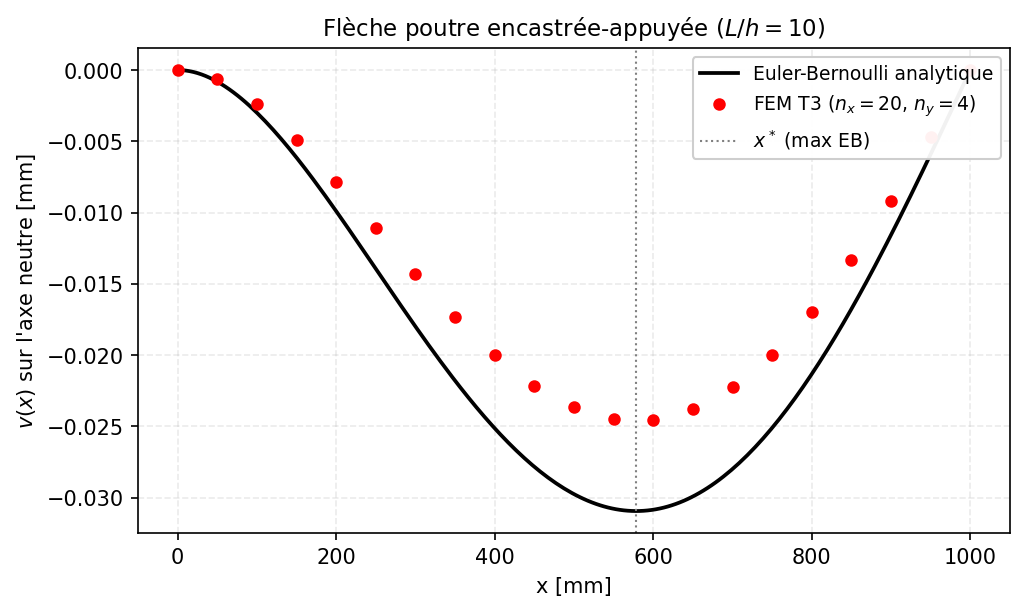
\includegraphics[width=0.84\linewidth]{figures/beam_deflection.png}
\caption{Profil de la flèche $v(x)$ sur l'axe neutre. La visualisation
\texttt{plotMesh()} demandée par le sujet est utilisée pour la déformée
(fig.~\ref{fig:postproc}).}
\label{fig:beam-deflection}
\end{figure}

\begin{figure}[!ht]
\centering
\begin{subfigure}[b]{0.49\linewidth}\centering
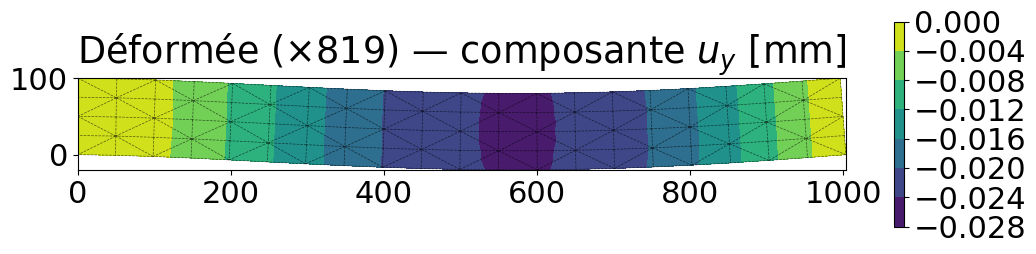
\includegraphics[width=\linewidth]{figures/beam_deformed.png}
\caption{Déformée amplifiée, composante $u_y$.}
\end{subfigure}\hfill
\begin{subfigure}[b]{0.49\linewidth}\centering
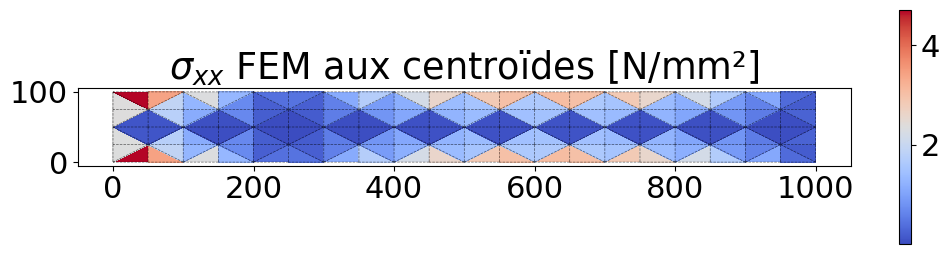
\includegraphics[width=\linewidth]{figures/sigma_field.png}
\caption{Carte $\sigma_{xx}$ aux centroïdes.}
\end{subfigure}
\caption{Post-traitement de la poutre encastrée-appuyée
($L/h=10$, T3 $20\!\times\!4$). La déformée montre la cuvette
caractéristique du \emph{propped cantilever}, avec un maximum de flèche
autour de $x\approx 0.58\,L$. La carte $\sigma_{xx}$ fait apparaître
la flexion attendue\,: compression supérieure à l'encastrement,
traction inférieure.}
\label{fig:postproc}
\end{figure}

\subsection{Étude paramétrique de l'élancement $L/h$}
À charge totale et maillage fixés ($n_x{=}20,\,n_y{=}4$), $h$ varie pour
balayer une poutre épaisse ($L/h=2$) jusqu'à très élancée ($L/h=100$).
La référence est la flèche EB recalculée avec le $h$ courant.

\begin{figure}[!ht]
\centering
\begin{minipage}[b]{0.55\linewidth}\centering
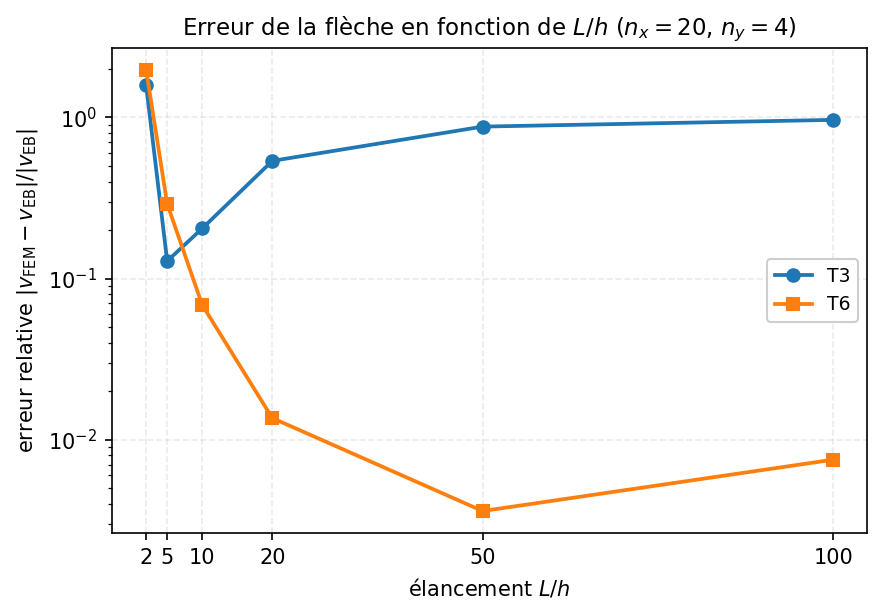
\includegraphics[width=\linewidth]{figures/err_vs_slenderness.png}
\end{minipage}\hfill
\begin{minipage}[b]{0.43\linewidth}\centering\small
\renewcommand{\arraystretch}{1.15}
\begin{tabular}{rrr}
\toprule
$L/h$ & err.\ T3 & err.\ T6 \\ \midrule
2     & 158\,\%  & 197\,\%  \\
5     & ~13\,\%  & ~29\,\%  \\
10    & ~20\,\%  & ~~7\,\%  \\
20    & ~54\,\%  & ~~1.4\,\% \\
50    & ~88\,\%  & ~~0.36\,\%\\
100   & ~97\,\%  & ~~0.75\,\%\\
\bottomrule
\end{tabular}
\end{minipage}
\caption{Erreur relative de la flèche $v(L/2)$ en fonction de
l'élancement. À $L/h=2$ et~5 la poutre est trop épaisse pour qu'EB soit
encore valide (l'écart est alors de modèle, pas FEM). Dès
$L/h\geq 10$, T3 explose (locking) tandis que T6 reste sous le pourcent.}
\label{fig:slenderness}
\end{figure}

% =========================================================================
\section{Convergence en $h$}

Mesurer l'erreur contre $v_\text{EB}$ sous-estime les vraies pentes de
convergence\,: la solution 2D élasticité diffère structurellement d'EB
d'environ 7\,\% à $L/h=10$ par effets de Poisson et de cisaillement
réel. On utilise donc une référence T6 ultra-fine
($n_x{=}320,\,n_y{=}64$, $\sim\!8\!\times\!10^4$ nœuds)\,:
$v_\text{ref} = -3.1959\!\times\!10^{-2}$~mm,
$v_\text{EB} = -2.9762\!\times\!10^{-2}$~mm, soit un écart de modèle
de 6.87\,\%. On raffine ensuite uniformément avec
$\text{hf}\in\{1,2,4,8\}$ et on ajuste
$\log(\text{err}) = p\log(h_\text{carac}) + b$.

\begin{figure}[!ht]
\centering
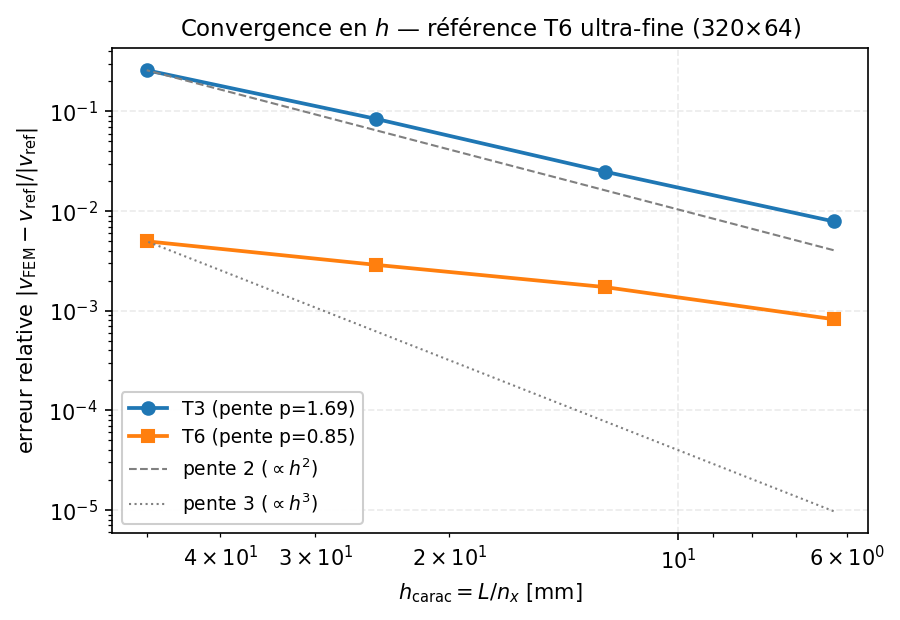
\includegraphics[width=0.7\linewidth]{figures/convergence_h.png}
\caption{Convergence en $h$ par rapport à la référence T6 ultra-fine.
T3 atteint $p\!\approx\!1.83$, proche du $p=2$ idéal mais légèrement
dégradé par le locking résiduel à $L/h=10$. T6 a une erreur
$\sim\!30\times$ plus faible à maillage égal\,; sa pente apparente est
plus modeste car son erreur résiduelle approche celle de la référence
elle-même.}
\label{fig:convh}
\end{figure}

% =========================================================================
\section{Analyse modale}

On résout $K\boldsymbol{\phi}_n = \omega_n^2 M\boldsymbol{\phi}_n$ sur les DDL libres. Les
fréquences analytiques d'EB pour propped cantilever proviennent des
racines $\beta_n L$ de $\tan(\beta L)=\tanh(\beta L)$\,:
$\omega_n = (\beta_n L)^2\sqrt{EI/(m_\text{lin} L^4)}$ avec
$m_\text{lin}=\rho\,t\,h$. Les valeurs propres SciPy sont multipliées
par $10^3$ pour convertir le système mixte mm-N-kg en rad/s.

\begin{table}[!ht]
\centering\small
\renewcommand{\arraystretch}{1.15}
\begin{tabular}{cccccc}
\toprule
mode & $f_\text{EB}$ [Hz] & $f_\text{T3}$ [Hz] & err.\ T3 &
                              $f_\text{T6}$ [Hz] & err.\ T6\\
\midrule
1 & 10.82 & 12.12 & $+12.0\,\%$ & 10.43 & $-3.6\,\%$\\
2 & 35.07 & 37.04 & $+5.6\,\%$  & 31.87 & $-9.1\,\%$\\
3 & 73.16 & 38.30 & $-47.6\,\%$ & 38.24 & $-47.7\,\%$\\
4 & 125.1 & 71.99 & $-42.5\,\%$ & 61.74 & $-50.6\,\%$\\
5 & 190.9 & 114.2 & $-40.2\,\%$ & 97.36 & $-49.0\,\%$\\
\bottomrule
\end{tabular}
\caption{Cinq premières fréquences propres ($n_x{=}20,\,n_y{=}4$). Sur
les deux modes de flexion fondamentaux, T6 est nettement plus proche
de EB. T3 surestime la rigidité, ce qui est la signature du locking en
dynamique. Au-delà du mode~2, le maillage 2D capte des modes de
cisaillement et de traction-compression absents de la suite EB\,:
les écarts d'environ $-50\,\%$ ne sont \emph{pas} un défaut FEM.}
\label{tab:modal}
\end{table}

% =========================================================================
\section{Diagnostic du piège FEM}\label{sec:locking}

\subsection{Origine du shear locking}
En flexion pure d'une poutre élancée, le champ exact 2D est
$u(x,y)=-\theta(x)\,\bar y$, $v(x,y)=v_0(x)$ avec $v_0' = \theta$, ce
qui annule exactement le cisaillement\,:
$\gamma_{xy} = \partial u/\partial y + \partial v/\partial x
= -\theta + v_0' = 0$.

Sur un T3 (déplacement linéaire), la cinématique ne peut pas
représenter simultanément $\theta$ linéaire et $v_0$ quadratique. Un
cisaillement parasite apparaît mécaniquement,
$\gamma_{xy}^\text{para}\sim h\,v_0''(x)$. Le ratio des énergies vaut
\[
\frac{W_\text{shear}^\text{para}}{W_\text{flexion}}
\;\sim\;\Big(\frac{L}{h}\Big)^{2},
\]
qui diverge quand la poutre s'amincit. La pénalité de cisaillement
domine alors $K$, l'élément devient artificiellement trop raide en
flexion et la flèche est sous-estimée. C'est le shear locking. La
signature numérique est exactement celle de la fig.~\ref{fig:slenderness}\,:
erreur T3 croissante avec $L/h$ et plafonnant près de 100\,\%.

\subsection{Évaluation T6}
Le T6, étant quadratique, peut représenter le terme $u\propto x\,\bar y$
nécessaire à $\gamma_{xy}=0$ exact. Le locking est donc éliminé en
pratique\,: erreur T6 sous le pourcent dès $L/h\geq 10$
(table~\ref{fig:slenderness}). La fig.~\ref{fig:locking} confirme cette
analyse. À $L/h=50$, raffiner $n_y$ ne réduit pas l'erreur T3
(plateau à 88\,\% même avec $n_y=16$), tandis que T6 atteint 0.4\,\%
dès $n_y=2$. \textbf{Le locking est intrinsèque à l'élément, pas à la
résolution.}

\begin{figure}[!ht]
\centering
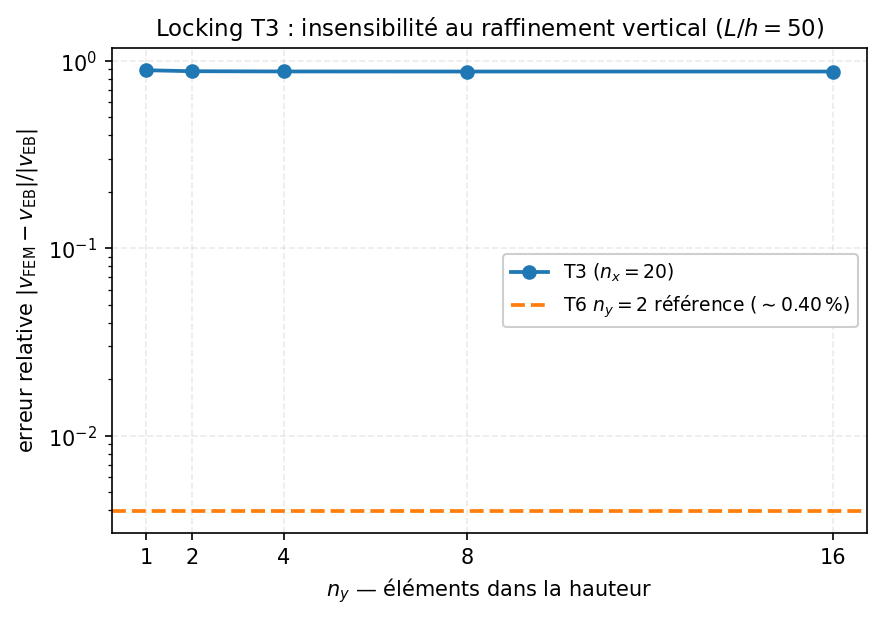
\includegraphics[width=0.7\linewidth]{figures/locking_demo.png}
\caption{Sensibilité du locking T3 à $n_y$ pour $L/h{=}50$ et $n_x{=}20$.
Le plateau confirme qu'un raffinement seul ne sauve pas T3\,: il faut
changer d'élément.}
\label{fig:locking}
\end{figure}

\subsection{Alternatives proposées}
Si l'on devait rester en T3, plusieurs voies sont classiques.

\begin{itemize}\setlength\itemsep{0.5pt}
\item \textbf{Sous-intégration sélective} (SRI). Standard sur Q4,
mais inapplicable à T3 qui est déjà à 1 point.
\item \textbf{B-bar} (Hughes 1980). Projection de $\gamma_{xy}$ sur un
sous-espace réduit avant le calcul de $K$, peu invasive, à valider sur
le patch test.
\item \textbf{MINI} (T3 enrichi d'une bulle interne). Restaure la
richesse cinématique au prix d'un DDL interne, condensable
statiquement.
\item \textbf{Reissner-Mindlin mixte}. DDL rotation indépendant,
plus structurel et soumis à la condition LBB.
\item \textbf{DKT} (Discrete Kirchhoff Triangle). Impose
$\gamma_{xy}=0$ aux arêtes mais reste spécifique au cadre plaque.
\end{itemize}

Pour ce projet, le choix retenu est T6\,: c'est la voie la plus simple,
déjà validée et sans surcoût notable sur les maillages typiques.

% =========================================================================
\section{Conclusion}

L'extension T3 vers T6 a été codée et validée par patch test à
$\sim 10^{-19}$ sur géométrie distordue, soit quatre ordres en dessous
du critère $10^{-15}$ du sujet. Sur la poutre encastrée-appuyée, T6
reproduit la flèche analytique d'Euler-Bernoulli à mieux que 1\,\% pour
$L/h\geq 20$, là où T3 atteint près de 100\,\% d'erreur, le shear
locking étant la cause et T6 le remède naturel. La convergence en $h$,
mesurée contre une référence T6 ultra-fine, donne une pente proche
de~1.8 pour T3\,; T6 fait 30 fois mieux à maillage équivalent.
L'analyse modale confirme la même hiérarchie sur les modes de flexion.
Le notebook reproductible et toutes les figures sont disponibles dans
le dépôt référencé en en-tête.

\end{document}
